\begin{esercizio}%[(07/02/2018 n°1)]
   An atom has a nucleus of charge $Z$ and one electron. The nucleus has radius $R$ inside which the charge is distributed. Assuming that the effect of the finite size of the nucleus can be described by the following potential:
   \begin{equation*}
      V(r)=
      \begin{dcases}
         -\frac{Z e^2}{R} \frac{r}{R} & \text{for } r<R\\
         -\frac{Z e^2}{r} & \text{for } r \geq R
      \end{dcases}
   \end{equation*}
   \begin{enumerate}[label=\alph*), leftmargin=0.6cm]
      \item Use perturbation theory to calculate the first order correction to the ground state for $Z=8$ and $A=16$. (It is known that $R=R_0A^{\frac{1}{3}}$ with $R_0=1.2 \cdot 10^{-15} \; \rm m=1.2 \; fm$)
      \item Do you expect perturbation theory to be more valid for larger $A$?\footnotemark\;Justify.
   \end{enumerate}
   Hint:
   \begin{gather*}
      E_1^{(0)}=-\frac{Z^2 e^2}{2a_0}
      \qq{with}
      a_0=\frac{\hbar^2}{mc^2}
      \qq{,}
      \frac{R^2}{2a_0}=13.6 \text{ eV}
      \\
      R_{1,0}=2\qty( \frac{Z}{a_0} )^{\frac{3}{2}} a^{-Zr/a_0}
   \end{gather*}
\end{esercizio}
\begin{soluzione}
   \footnotetext{Questa richiesta ci sta implicitamente dicendo di fissare il valore di $Z$ e far variare soltanto $A$.}
   Per prima cosa è conveniente, quando possibile, riportare in un grafico l'andamento del potenziale. In questo caso il potenziale assume la forma di una retta con pendenza negativa fino a $r=R$ (cioè fino alla \textit{size} del nucleo), dopodiché diventa un'iperbole. Pertanto, graficamente il potenziale apparirà come segue:

   \begin{figure}[H]
      \centering
      \begin{tikzpicture}[scale=1.6]
         \draw[->] (0,-2.2) -- (0,1) node[above] {$V$};
         \draw[->] (-1,0) -- (4.2,0) node[right] {$r$};
         \draw[dotted] (1,-1) -- (1,0) node[above] {$R$};
         \draw[thick,dashed,gray] plot[smooth,domain=0.5:1] (\x,-1/\x) -- plot[smooth,domain=1:2] (\x,-\x);
         \draw[thick,red!60!black] plot[smooth,domain=0:1] (\x,-\x) -- plot[smooth,domain=1:4] (\x,-1/\x);
      \end{tikzpicture}
   \end{figure}

   Osserviamo adesso che il sistema in esame è un atomo idrogenoide, pertanto il problema si può affrontare nella stessa maniera con cui trattiamo l'atomo di idrogeno avendo però carica $Z$ diversa da 1.
   
   Osserviamo inoltre che per $r \geq R$ il potenziale $V(r)$ assume proprio la forma del potenziale dell'atomo idrogenoide, per cui la hamiltoniana sarà quella dell'atomo idrogenoide, che ricordiamo essere

   \begin{equation*}
      H_{\rm idrogenoide}
      =\frac{p^2}{2m} - \frac{Ze^2}{r}
   \end{equation*}

   Quello che vogliamo è che questa sia la nostra $H_0$,\footnote{Osserviamo che tale hamiltoniana ha una parte di potenziale, ma ciò non ci spaventa perché conosciamo esattamente tale problema.} in quanto ne conosciamo autovalori ed autofunzioni. \E in quest'ottica che capiamo come impostare il problema: nella regione 'nuova', cioè quella per $r<R$ in cui è presente il potenziale dovuto alla distribuzione di carica nella finite size del nucleo, tale potenziale deve essere considerato come perturbazione rispetto al potenziale dell'atomo idrogenoide, per cui dobbiamo esprimerlo in modo da ottenere il potenziale di $H_0$ più un termine perturbativo. Scriviamo dunque la hamiltoniana per la regione $r<R$:
   
   \begin{equation}
      H=\frac{p^2}{2m} - \frac{Ze^2}{R} \frac{r}{R}
      \label{eq:hamiltoniana_atomo_idrogenoide}
   \end{equation}

   Concentriamoci sul termine di potenziale e riscriviamolo aggiungendo e sottraendo il termine $\frac{Z e^2}{r}$:

   \begin{equation*}
      -\frac{Ze^2}{R} \frac{r}{R}
      =-\frac{Ze^2}{R} \frac{r}{R} + \frac{Z e^2}{r} - \frac{Z e^2}{r}
   \end{equation*}

   Riordinando i termini e inserendoli in \eqref{eq:hamiltoniana_atomo_idrogenoide} possiamo riscrivere quest'ultima come

   \begin{equation*}
      H
      =\frac{p^2}{2m} - \frac{Z e^2}{r} - \frac{Ze^2}{R} \frac{r}{R} + - \frac{Z e^2}{r}
      =H_0 + V'
   \end{equation*}
   
   dove $H_0$ è la hamiltoniana dell'atomo idrogenoide e $V'$ è il termine di perturbazione, il quale può essere riscritto come

   \begin{equation*}
      V'
      =-\frac{Ze^2}{R} \frac{r}{R} + \frac{Z e^2}{r}
      =-\frac{Z e^2}{R} \qty( \frac{r}{R} - \frac{R}{r} )
   \end{equation*}

   Il problema chiede qual è la correzione al ground state al primo ordine. Essa è data dall'elemento di matrice di $V'$ rispetto al ground state imperturbato, cioè rispetto a $\ket*{1,0,0}$. In formule\footnote{Notiamo che l'integrale radiale è esteso fino a $r=R$. Il motivo è che la perturbazione è nulla per $r \geq R$.}:
   
   \begin{gather*}
      \delta E_1^{(1)}
      =\mel*{1,0,0}{V'}{1,0,0}
      =\int_{0}^{R} \dd{r} r^2 \int \dd{\Omega} \psi^*_{1,0,0}(r,\vartheta,\varphi) V'(r) \psi_{1,0,0}(r,\vartheta,\varphi)
      =
      \\
      =-\int_{0}^{R} \dd{r} r^2 \int \dd{\Omega} |Y_{0,0}(\vartheta,\varphi)|^2 |R_{1,0}(r)|^2 \frac{Z e^2}{R} \qty( \frac{r}{R} - \frac{R}{r} )
   \end{gather*}

   dove nell'ultimo passaggio abbiamo esplicitato il potenziale e la funzione d'onda.

   L'espressione della parte radiale è fornita dal testo, mentre per la parte angolare si ha

   \begin{equation*}
      \int \dd{\Omega} |Y_{0,0}(\vartheta,\varphi)|^2
      =\frac{1}{4\pi} \int \dd{\Omega}
      =\frac{1}{4\pi} 4\pi
      =1
   \end{equation*}

   In definitiva possiamo riscrivere

   \begin{gather*}
      \mel*{1,0,0}{V'}{1,0,0}
      =-\int_{0}^{R} \dd{r} r^2 4 \qty( \frac{Z}{a_0} )^3 e^{-2Zr/a_0} \frac{Ze^2}{R} \qty( \frac{r}{R} - \frac{R}{r} )
      =\\
      =-\frac{Z e^2}{R} \qty( \frac{Z}{a_0} )^3 4 \int_{0}^{R} \dd{r} r^2 \qty( \frac{r}{R} - \frac{R}{r} ) e^{2Zr/a_0}
   \end{gather*}

   Effettuiamo ora il cambio di variabile

   \begin{equation*}
      x=\frac{2Zr}{a_0}
      \implies
      r=\frac{a_0}{2Z}x
      \implies
      \dd{r}=\frac{a_0}{2Z} \dd{x}
   \end{equation*}

   che modifica l'intervallo di integrazione da $[0,R]$ in $[0,\alpha]$, con $\alpha=2ZR/a_0$. Dopo alcuni passaggi si giunge all'integrale

   \begin{equation}
      \frac{Ze^2}{2R} \int_{0}^{\alpha} \dd{x} e^{-x} \qty( \alpha x - \frac{x^3}{\alpha} )
      \label{eq:integrale_dopo_sostituzione}
   \end{equation}

   Questi integrali vanno risolti per parti. In particolare si trova che

   \begin{gather*}
      \int_{0}^{\alpha} \dd{x} e^{-x} x
      =-e^{-\alpha} (\alpha + 1) + 1
      \\[0.1cm]
      \int_{0}^{\alpha} \dd{x} e^{-x} x^3
      =-e^{-\alpha} (\alpha^3 + 3\alpha^2 + 6\alpha + 6) + 6
   \end{gather*}

   Da cui, inserendo tali risultati nell'espressione \eqref{eq:integrale_dopo_sostituzione}, otteniamo

   \begin{equation*}
      \frac{Ze^2}{2R} \int_{0}^{\alpha} \dd{x} e^{-x} \qty( \alpha x - \frac{x^3}{\alpha} )
      =\frac{Z e^2}{2R} \qty[ \alpha - \frac{6}{\alpha} + e^{-\alpha}\qty( 2\alpha + 6 + \frac{6}{\alpha} ) ]
   \end{equation*}

   Osserviamo adesso che il coefficiente a moltiplicare davanti la parentesi quadra può essere riscritto come

   \begin{equation*}
      \frac{Z e^2}{2R}
      =\frac{Z^2 e^2}{a_0} \frac{a_0}{2ZR}
   \end{equation*}

   Il primo fattore è uguale all'opposto del doppio dell'energia del ground state imperturbato, mentre il secondo termine, per come abbiamo definito $\alpha$, è uguale proprio ad $\alpha^{-1}$. In definitiva possiamo scrivere:

   \begin{equation*}
      \frac{Z e^2}{2R}
      =-2E_1^{(0)} \frac{1}{\alpha}
   \end{equation*}

   e quindi avremo

   \begin{equation}
      \frac{Z e^2}{2R} \qty[ \alpha - \frac{6}{\alpha} + e^{-\alpha}\qty( 2\alpha + 6 + \frac{6}{\alpha} ) ]
      =-2E_1^{(0)} \qty[ 1 - \frac{6}{\alpha^2} + e^{-\alpha}\qty( 2 + \frac{6}{\alpha} + \frac{6}{\alpha^2} ) ]
      \label{eq:risultato_integrale_per_parti_con_sostituzione_hint}
   \end{equation}

   Arrivati a questo punto possiamo rispondere alla domanda a): abbiamo infatti trovato la correzione al primo ordine allo stato fondamentale, e adesso dobbiamo trovarla in particolare per $Z=8$ ed $A=16$. Cerchiamo quindi di stimare $\alpha$ per questi valori. Sfruttando il fatto che $R=R_0A^{\frac{1}{3}}$ riscriviamo $\alpha$ come

   \begin{equation*}
      \alpha
      =\frac{2ZR}{a_0}
      =\frac{3R_0}{a_0} Z A^{\frac{1}{3}}
   \end{equation*}

   dove abbiamo lasciato $A$ e $Z$ non espressi in modo da avere una formula che vale per qualsiasi atomo. Possiamo riscrivere ancora:
   
   \begin{equation*}
      \frac{3R_0}{a_0} Z A^{\frac{1}{3}}
      =\gamma A^{\frac{1}{3}}
   \end{equation*}

   dove\footnote{Questo valore si trova per $Z=8$. Il motivo per cui sostituiamo subito $Z$ è che il problema chiede dei ragionamenti su $A$, per cui possiamo considerare $Z$ fissato.} $\gamma=3.6 \cdot 10^{-4}$. Segue che per $A=16$ risulta $\alpha \approx 10^{-3} \ll 1$.
   
   Possiamo sfruttare il fatto che $\alpha \ll 1$ per avere un'espressione analitica: sviluppando in serie di Taylor l'esponenziale otteniamo:
   
   \begin{equation*}
      e^{-\alpha}
      =1 - \alpha + \frac{\alpha^2}{2}
   \end{equation*}

   dove ci siamo fermati al secondo ordine. Prestiamo attenzione a questo fatto: il motivo per cui ci siamo fermati al secondo ordine piuttosto che al primo è che nelle parentesi quadre dell'espressione \eqref{eq:risultato_integrale_per_parti_con_sostituzione_hint} abbiamo termini fino all'ordine $\alpha^{-2}$. Inserendo quindi tale espansione otteniamo

   \begin{gather*}
      1 - \frac{6}{\alpha^2} + e^{-\alpha}\qty( 2 + \frac{6}{\alpha} + + \frac{6}{\alpha^2} )
   =1 - \frac{6}{\alpha^2} + \qty( 1 - \alpha + \frac{\alpha^2}{2} )\qty( 2 + \frac{6}{\alpha} + \frac{6}{\alpha^2} )
   =\\
   =1 - \frac{6}{\alpha^2} + 2 +\frac{6}{\alpha} + \frac{6}{\alpha^2} - 2\alpha - 6 - \frac{6}{\alpha} + \alpha^2 + 3\alpha + 3
   =\alpha^2 + \alpha \approx \alpha
   \end{gather*}
   
   dove nell'ultimo passaggio trascuriamo il termine $\alpha^2$ in quanto $\alpha \ll 1$.

   In definitiva abbiamo trovato un'espressione analitica semplice per la correzione al primo ordine al ground state, che è

   \begin{equation*}
      \delta E_1^{(1)}=-2 \alpha E_1^{(0)}
   \end{equation*}

   da cui si trova, per $Z=8$ $A=16$,

   \begin{equation*}
      \delta E_1^{(1)}=1.6 \text{ eV}
   \end{equation*}

   A questo punto passiamo al quesito b). Per capire se la teoria perturbativa è valida, dobbiamo verificare che si abbia

   \begin{equation*}
      \biggl| \frac{ \delta E_1^{(1)} }{ E_1^{(0)} - E_{2}^{(0)} } \biggr| \ll 1
   \end{equation*}

   Abbiamo già calcolato $\delta E_1^{(1)}$, passiamo al calcolo di $E_1^{(0)} - E_{2}^{(0)}$: ricordando che per un atomo idrogenoide i livelli energetici sono dati da

   \begin{equation*}
      E_n=-\frac{Z^2 e^2}{2 a_0 n^2}
   \end{equation*}

   avremo

   \begin{equation*}
      E_1^{(0)} - E_{2}^{(0)}
      =-\frac{Z^2 e^2}{2 a_0} \qty( 1 - \frac{1}{4} )
      =-\frac{3}{4} \frac{Z^2 e^2}{2 a_0}
      =-\frac{3}{4} E_1^{(0)}
   \end{equation*}

   In definitiva:

   \begin{equation*}
      \biggl| \frac{ \delta E_1^{(1)} }{ E_1^{(0)} - E_{2}^{(0)} } \biggr|
      =\biggl| \frac{ -2 \alpha E_1^{(0)} }{ -\frac{3}{4} E_1^{(0)} } \biggr|
      =\frac{8}{3} \alpha
   \end{equation*}

   Ricordiamo che abbiamo trovato

   \begin{equation*}
      \alpha=\gamma A^{\frac{1}{3}}
   \end{equation*}

   da cui sembrerebbe che all'aumentare di $A$ la teoria perturbativa sia sempre meno valida. Tuttavia, sostituendo il valore di $\gamma$, troviamo che

   \begin{equation*}
      \frac{8}{3} \cdot 3.6 \cdot 10^{-4} A^{\frac{1}{3}} \ll 1
      \implies
      A^{\frac{1}{3}} \ll 10^3
      \implies
      A \ll 10^9
   \end{equation*}

   il che significa che, per i valori che $A$ assume in natura, la teoria perturbativa è valida.
\end{soluzione}

\newpage
\setcounter{equation}{0}

\begin{esercizio}%[(13/07/2018 n°2)]
   A two-level system is described by the hamiltonian
   \begin{equation*}
      H_0=
      \begin{pmatrix}
         \Omega & 0\\
         0 & 3\Omega
      \end{pmatrix}
      \hbar
   \end{equation*}
   The system is in the excited state. At time $t=0$ the following perturbation turned on for a long time $T$:
   \begin{equation*}
      H_1=
      \begin{pmatrix}
         0 & \Omega e^{i\omega t}\\
         \Omega e^{-i\omega t} & 0\\
      \end{pmatrix}
      \hbar
   \end{equation*}
   \begin{enumerate}[label=\alph*), leftmargin=0.6cm]
      \item Find the transition amplitude to the ground state at $t>T$.
      \item Is there a valure of $\omega/\Omega$ such that the probability to make transition reaches at most $0.5$?
   \end{enumerate}
\end{esercizio}
\begin{soluzione}
   In questo problema abbiamo un sistema a due livelli, quindi abbiamo solo il ground state e uno stato eccitato. Il sistema si trova nello stato eccitato, quindi l'unica transizione che può compiere è verso il ground state. Per studiare il sistema dobbiamo studiare il problema agli autovalori
   
   \begin{equation*}
      H_0\ket*{\varphi_n^{(0)}}
      =E_n\ket*{\varphi_n^{(0)}}
      \qq{con}
      n=1,2
   \end{equation*}

   In generale per trovare autovalori e autostati dovremmo diagonalizzare la matrice. In questo caso la matrice è già in forma diagonale, per cui possiamo dire subito che gli autostati sono:

   \begin{eqnarray*}
      \text{ground state} & \varphi_1^{(0)}
      =
      \begin{pmatrix}
         1\\
         0
      \end{pmatrix}
      & \text{con energia } E_1=\hbar \Omega
      \\[0.1cm]
      \text{excited state} & \varphi_2^{(0)}
      =
      \begin{pmatrix}
         0\\
         1
      \end{pmatrix}
      & \text{con energia } E_2=3\hbar \Omega
   \end{eqnarray*}

   Svolgiamo ora il punto a). L'ampiezza di transizione $d_{2 \to 1}$ dallo stato eccitato verso il ground state è data da
   
   \begin{equation}
      d_{2 \to 1}
      =-\frac{i}{\hbar} \int_{0}^{T} \dd{t} e^{i\omega_{1,2} t} V_{1,2}
      \label{eq:ampiezza_di_transizione}
   \end{equation}

   Notiamo che l'integrazione è estesa da $0$, tempo in cui si accende la perturbazione, a $T$, tempo in cui si spegne. Il motivo è che il testo ci chiede di calcolare la probabilità per un tempo $t>T$, dunque l'integrale è non nullo fino a $t=T$.

   Osserviamo adesso che

   \begin{equation*}
      V_{1,2}
      =\mel*{\varphi_1^{(0)}}{H_1}{\varphi_2^{(0)}}
      =
      \begin{pmatrix}
         1 & 0
      \end{pmatrix}
      \begin{pmatrix}
         0 & \hbar \Omega e^{i\omega t}\\
         \hbar \Omega e^{-i\omega t} & 0\\
      \end{pmatrix}
      \begin{pmatrix}
         0\\
         1
      \end{pmatrix}
      =
      \begin{pmatrix}
         1 & 0
      \end{pmatrix}
      \begin{pmatrix}
         \hbar \Omega e^{i\omega t}\\
         0
      \end{pmatrix}
      =\hbar \Omega e^{i \omega t}
   \end{equation*}
   
   e

   \begin{equation*}
      \omega_{1,2}
      =\frac{E_1 - E_2}{\hbar}
      =\frac{\hbar \Omega - 3\hbar \Omega}{\hbar}
      =-2\Omega
   \end{equation*}

   Inserendo tali espressioni in \eqref{eq:ampiezza_di_transizione} possiamo riscrivere quest'ultima come

   \begin{equation}
      d_{2 \to 1}
      =-\frac{i}{\hbar} \int_{0}^{T} \dd{t} \hbar \Omega e^{i( \omega - 2\Omega ) t}
      =-\frac{\Omega}{\omega - 2\Omega} \qty[ e^{i(\omega - 2\Omega)T} - 1 ]
      \label{eq:ampiezza_di_transizione_riscritta}
   \end{equation}

   Passiamo alla domanda b). Il testo chiede qual è il valore del rapporto $\omega/\Omega$ tale che la probabilità di transizione valga al massimo $0.5$. Innanzitutto per calcolare la probabilità di transizione è sufficiente considerare il modulo quadro della \eqref{eq:ampiezza_di_transizione_riscritta}:

   \begin{equation*}
      P_{2 \to 1}
      =| d_{2 \to 1} |^2
      =\frac{\Omega^2}{(\omega - 2\Omega)^2} \qty| e^{i(\omega - 2\Omega)T} - 1 |^2
   \end{equation*}
   
   Svolgiamo il prodotto ricordando che per un numero complesso si ha $|z|^2=z^*z$

   \begin{gather*}
      P_{2 \to 1}
      =\frac{\Omega^2}{(\omega - 2\Omega)^2} \qty[ e^{-i(\omega - 2\Omega)T} - 1 ] \qty[ e^{i(\omega - 2\Omega)T} - 1 ]=
      \\
      =\frac{\Omega^2}{(\omega - 2\Omega)^2} \qty[ 1 - e^{i(\omega - 2\Omega)T} - e^{-i(\omega - 2\Omega)T} + 1 ]
   \end{gather*}

   Ricordando inoltre che

   \begin{equation*}
      \cos{\alpha}=\frac{e^{i\alpha} + e^{-i\alpha}}{2}
   \end{equation*}

   otteniamo

   \begin{equation*}
      P_{2 \to 1}
      =\frac{2\Omega^2}{(\omega - 2\Omega)^2} \Bigl\{ 1 - \cos{ \bigl[ (\omega - 2\Omega) T \bigr] } \Bigr\}
   \end{equation*}

   Sfruttando ora la formula di bisezione del seno

   \begin{equation*}
      \sin{\qty( \frac{\alpha}{2} )}
      =\pm \sqrt{ \frac{1 - \cos{\alpha}}{2} }
   \end{equation*}

   Possiamo riscrivere ancora

   \begin{equation*}
      P_{2 \to 1}
      =\frac{4\Omega^2}{(\omega - 2\Omega)^2} \sin^2{ \qty[ \frac{ (\omega - 2\Omega) T }{2} ] }
   \end{equation*}

   Osserviamo che siccome il testo ci chiede delle condizioni sui valori superiori (\textit{at most} $0.5$), possiamo considerare la seguente catena di disuguaglianze:
   
   \begin{equation*}
      \frac{4\Omega^2}{(\omega - 2\Omega)^2} \sin^2{ \qty[ \frac{ (\omega - 2\Omega) T }{2} ] }
      \leq \frac{4\Omega^2}{(\omega - 2\Omega)^2}
      \leq \frac{1}{2}
   \end{equation*}

   e in particolare l'ultima disuguaglianza può essere riscritta come
   
   \begin{equation*}
      8\Omega^2 \leq \omega^2 + 4\Omega^2 - 4\omega\Omega
   \end{equation*}

   visto che dobbiamo trovare una condizione in termini del rapporto $\omega/\Omega$, dividiamo per $\Omega^2$:

   \begin{equation*}
      \qty( \frac{\omega}{\Omega} )^2 - 4\qty( \frac{\omega}{\Omega} ) - 4 \geq 0
      \implies
      \frac{\omega}{\Omega} \geq 2 ( 1 + \sqrt{2} ) \simeq 4.83
   \end{equation*}
\end{soluzione}

\newpage
\setcounter{equation}{0}

\begin{esercizio}
   An electron is under the potential
   \begin{equation*}
      V'(x)=
      \begin{dcases}
         V_0 \sin{\qty( \frac{\pi}{L} x )} & \text{for } 0<x<L\\
         +\infty & \text{otherwhise}\\
      \end{dcases}
   \end{equation*}
   \begin{enumerate}[label=\alph*), leftmargin=0.6cm]
      \item Calculate the energy levels employing first-order perturbation theory.
      \item What is the condition $V_0$ has to satisfy for perturbation theory to be valid for $n=1$ level? Is it valid for $V_0=0.4$ eV and $L=0.2$ nm for $n=1$ level and/or for all the $n$ energy levels? (Explain)
      \item At $t>0$ the potential becomes
      \begin{equation*}
         V''(x,t)=V_0 \sin{\qty( \frac{\pi}{L} x )}\cos{(\omega t)}
      \end{equation*}
      Calculate the transition probability for $n=1$ to $n=3$ at time $T$ at the value of $\omega$ where it is maximal.
      \item For $L=0.2$ nm and $V_0=0.4$ eV is time-dependent perturbation theory expected to be valid if $T=\frac{15 \pi}{\omega_{1,3}}$?
   \end{enumerate}
   Hint:
   \begin{gather*}
      \int_{0}^{L} \dd{y} \sin^2{\qty( \frac{n\pi}{L} y )} \sin{\qty( \frac{\pi}{L} y )}
      =\frac{L}{\pi} \frac{4n^2}{4n^2 - 1}
      \\[0.1cm]
      \int_{0}^{L} \dd{y} \sin{\qty( \frac{3\pi}{L} y )} \sin^2{\qty( \frac{\pi}{L} y )}
      =-\frac{8 L}{30 \pi}
   \end{gather*}
\end{esercizio}
\begin{soluzione}
   Per prima cosa rappresentiamo il potenziale prima che venga introdotta la dipendenza temporale:
   \begin{figure}[H]
      \centering
      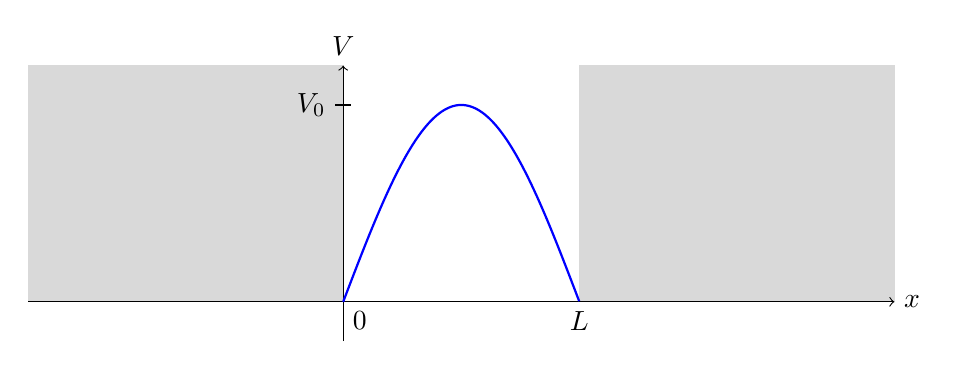
\begin{tikzpicture}
         \filldraw[gray!30!] (0,0) -- (0,3) -- (-4,3) -- (-4,0) -- cycle;
         \filldraw[gray!30!] (3,0) -- (3,3) -- (7,3) -- (7,0) -- cycle;
         \draw[->](-4,0) -- (7,0) node[right] {$x$};
         \draw[->](0,-0.5) -- (0,3) node[above] {$V$};
         \draw[domain=0:3, smooth, samples=200, thick, blue] plot (\x, {2.5*sin(pi/3*\x r)});
         \node[below right] at (0,0) {$0$};
         \node[below] at (3,0) {$L$};
         \draw (-0.1,2.5) node[left] {$V_0$} -- (0.1,2.5);
      \end{tikzpicture}
   \end{figure}
   Esso ha l'andamento di una sinusoide per $x \in [0,L]$, ed è infinito all'esterno (le regioni grigie in figura).

   Svolgiamo il quesito a). Per questo è sufficiente applicare la teoria perturbativa indipendente dal tempo. La hamiltoniana imperturbata di questo sistema è quella di una particella confinata in una buca, cioè
   
   \begin{equation*}
      H_0=K + U
      \qq{dove}
      U=
      \begin{cases}
         0 & \text{per } 0 < x < L\\
         \infty & \text{altrove}\\
      \end{cases}
   \end{equation*}
   
   Di questo sistema conosciamo le autofunzioni, le quali saranno le autofunzioni imperturbate e che sono date da\footnote{Attenzione! Le autofunzioni hanno questa espressione perché la particella si trova in una buca tra $0$ e $L$. Se la buca fosse stata estesa da $-L/2$ a $L/2$ (buca centrata all'origine), le autofunzioni avrebbero avuto un'altra espressione.}
   
   \begin{equation*}
      \psi_n^{(0)}(x)
      =\sqrt{\frac{2}{L}} \sin{\qty( \frac{n \pi}{L} x)}
      \qq{,}
      n=1,2,\ldots
   \end{equation*}

   e a cui sono associate rispettivamente le energie

   \begin{equation*}
      E_n^{(0)}
      =\frac{\hbar^2 \pi^2 n^2}{2mL^2}
      \qq{,}
      n=1,2,\ldots
   \end{equation*}

   Il potenziale
   
   \begin{equation*}
      V'=V_0\sin\qty( \frac{\pi}{L} x)
   \end{equation*}

   costituisce la perturbazione per questo sistema. A causa della presenza di questo, la correzione al primo ordine dell'energia dell'$n$-esimo stato è data da
   
   \begin{equation*}
      \delta E_n^{(1)}
      =\mel*{\psi_n^{(0)}}{V'}{\psi_n^{(0)}}
      =\int_{0}^{L} \dd{x} V'(x) |\psi_n^{(0)}(x)|^2
      =\frac{2V_0}{L} \int_{0}^{L} \dd{x} \sin{\qty( \frac{\pi}{L} x )} \sin^2{\qty( \frac{n\pi}{L} x )}
   \end{equation*}
   
   dove nell'ultimo passaggio abbiamo esplicitato il potenziale e l'autofunzione.

   Notiamo che l'integrale che figura è fornito come hint dal testo, per cui possiamo inserire direttamente il risultato:

   \begin{equation}
      \delta E_n^{(1)}
      =\frac{2V_0}{L} \frac{L}{\pi} \frac{4n^2}{4n^2 - 1}
      =\frac{V_0}{\pi} \frac{8n^2}{4n^2 - 1}
      \label{eq:correzione_al_primo_ordine_livelli_buca}
   \end{equation}
   
   Per rispondere infine alla domanda dobbiamo calcolare le energie corrette al primo ordine, le quali sono date da

   \begin{equation*}
      E_n^{(1)}
      =E_n^{(0)} + \delta E_n^{(1)}
      =\frac{\hbar^2 \pi^2 n^2}{2mL^2} + \frac{V_0}{\pi} \frac{8n^2}{4n^2 - 1}
      \qq{,}
      n=1,2,\ldots
   \end{equation*}

   Passiamo al punto b). Cerchiamo quindi qual è la condizione che $V_0$ deve soddisfare affinché la teoria perturbativa sia valida per $n=1$: per essere valida, il rapporto tra la correzione al primo ordine e la differenza tra i livelli vicini deve essere molto minore di uno:
   
   \begin{equation*}
      \biggl| \frac{\delta E_1^{(1)}}{ E_1^{(0)} - E_2^{(0)} } \biggr| \ll 1
   \end{equation*}

   Ovvero, ricordando che

   \begin{equation*}
      E_1^{(0)} - E_2^{(0)}
      =-3 \frac{\hbar^2 \pi^2}{2 m L^2}
   \end{equation*}
   
   e sostituendo l'espressione \eqref{eq:correzione_al_primo_ordine_livelli_buca} per $n=1$,

   \begin{equation*}
      \qty| \frac{ \frac{8V_0}{3\pi} }{ -\frac{3 \hbar^2 \pi^2}{2 m L^2} } |
      =\frac{16 V_0 m L^2}{9 \hbar^2 \pi^3}
      \ll 1
      \implies
      V_0
      \ll \frac{9 \hbar^2 \pi^3}{16 m L^2}
   \end{equation*}

   Possiamo esprimere tale condizione in termini di $E_1^{(0)}$:

   \begin{equation*}
      V_0
      \ll \frac{9 \hbar^2 \pi^3}{16 m L^2}
      =\frac{\hbar^2 \pi^2}{2 m L^2} \frac{9 \pi}{8}
      =\frac{9 \pi}{8} E_1^{(0)}
   \end{equation*}

   Se $V_0$ soddisfa tale condizione, allora la teoria perturbativa è valida. Verifichiamo ora se è valida in particolare per $V_0=0.4$ eV e $L=0.2$ nm. Per fare ciò cerchiamo di esprimere tutte le quantità in elettronVolt e nanometri\footnote{In generale negli esercizi si hanno due casi: o le grandezze sono espresse in MeV e fm o eV e nm. In questo caso il testo fornisce le quantità in eV e nm, il che significa che esse sono delle quantità adeguate per il sistema.}, inoltre cerchiamo di far apparire la quantità $\hbar c$ che sappiamo valere 200 $\rm MeV \cdot fm$ o 200 $\rm eV \cdot nm$. Per fare ciò sfruttiamo il fatto che per la massa dell'elettrone si ha $m_e c^2 \approx 0.5 \; \rm MeV=0.5 \cdot 10^6 \; \rm eV$, fatto che ci suggerisce di moltiplicare e dividere per $c^2$:

   \begin{equation*}
      V_0
      \ll \frac{\hbar^2 \pi^2}{2 m L^2} \frac{9 \pi}{8}
      = \frac{(\hbar c)^2 \pi^2}{2 (m c^2) L^2} \frac{9 \pi}{8}
      =\rm \frac{4 \cdot 10^4 \; eV^2 \cdot nm^2 \, \pi^3 \, 9}{8 \cdot 2 \cdot 0.5 \cdot 10^6 \; eV \cdot 4 \cdot 10^{-2} \; nm^2}
      =\frac{\pi^3 \, 9}{8} \; eV
      =35 \; eV
   \end{equation*}

   Poiché il testo ci chiede di verificare la validità della teoria perturbativa per $V_0=0.4$ eV, troviamo che essa è valida per il livello con $n=1$.
   
   A questo punto dobbiamo controllare la validità anche per gli altri livelli di energia. Per fare ciò consideriamo il generico livello $n$-esimo e imponiamo la condizione di validità della teoria perturbativa per questo:
   
   \begin{gather*}
      \biggl| \frac{\delta E_n^{(1)}}{ E_n^{(0)} - E_{n + 1}^{(0)} } \biggr|
      =\qty| \frac{ \frac{V_0}{\pi} \frac{8n^2}{4n^2 - 1} }{ \frac{\hbar^2 \pi^2}{2 m L^2} \bigl[ n^2 - (n + 1)^2 \bigr] } |
      =\frac{ \frac{|V_0|}{\pi} \frac{8n^2}{4n^2 - 1} }{ \frac{\hbar^2 \pi^2}{2 m L^2} (2n + 1) }
      \ll 1
      \\
      \implies
      V_0 \ll \frac{\hbar^2 \pi^2}{32 m L^2} \qty( 4 - \frac{1}{n^2} ) ( 2n + 1 )
   \end{gather*}

   Sia il termine $4 - \frac{1}{n^2}$ che il termine $2n + 1$ sono funzioni crescenti di $n$, per cui tutto il termine a destra della disuguaglianza cresce all'aumentare di $n$. Ne segue che la teoria perturbativa è sempre più valida man mano che consideriamo $n$ maggiori.

   Passiamo alla richiesta c). Qui il potenziale cambia e ottiene una dipendenza dal tempo, quindi passiamo alla teoria perturbativa dipendente dal tempo. Il problema chiede di calcolare la proprietà di transizione dal livello con $n=1$ a quello con $n=3$ al tempo $T$ dove è massima. Questa è data da
   
   \begin{equation}
      d_{1 \to 3}
      =-\frac{i}{\hbar} \int_{0}^{T} \dd{t} e^{i \omega_{3,1} t} V''_{3,1}
      \label{eq:ampiezza_probabilit_da_3_a_1}
   \end{equation}

   dove

   \begin{equation*}
      \omega_{3,1}
      =\frac{E_3 - E_1}{\hbar}
      =\frac{4 \hbar \pi^2}{m L^2}
   \end{equation*}

   e

   \begin{gather*}
      V''_{3,1}
      =\mel*{\psi_3^{(0)}}{V''(x,t)}{\psi_1^{(0)}}
      =V_0 \cos{(\omega t)} \mel*{\psi_3^{(0)}}{\sin{ \qty( \frac{\pi}{L} x ) }}{\psi_1^{(0)}}=
      \\[0.1cm]
      =V_0 \cos{(\omega t)} \int_{0}^{L} \dd{x} \psi_3^{(0)}(x) \sin{ \qty( \frac{\pi}{L} x ) } \psi_1^{(0)}(x)
      =\frac{2V_0}{L} \cos{(\omega t)} \int_{0}^{L} \dd{x} \sin{ \qty( \frac{3\pi}{L} x ) } \sin^2{ \qty( \frac{\pi}{L} x ) }
   \end{gather*}

   Il risultato dell'integrale è fornito dall'hint, per cui possiamo subito scrivere

   \begin{equation*}
      V''_{3,1}
      =\frac{2V_0}{L} \cos{(\omega t)} \qty( - \frac{8 L}{30 \pi} )
      =-\frac{8 V_0}{15 \pi} \cos{(\omega t)}
   \end{equation*}

   Per inciso, notiamo che il problema chiede la probabilità di passare da $n=3$ a $n=1$ e non quella da $n=2$ a $n=1$ perché quest'ultima avrebbe dato luogo ad un integrale nullo per ragioni di parità.

   Esplicitando l'espressione di $V_{3,1}''$ in \eqref{eq:ampiezza_probabilit_da_3_a_1} otteniamo

   \begin{equation*}
      d_{1 \to 3}
      =\frac{i}{\hbar} \frac{8 V_0}{15 \pi} \int_{0}^{T} \dd{t} e^{i \omega_{3,1} t} \cos{(\omega t)}
   \end{equation*}

   Esprimendo il coseno come

   \begin{equation*}
      \cos{(\omega t)}
      =\frac{e^{i\omega t} - e^{i\omega t}}{2}
   \end{equation*}
   
   Possiamo riscrivere\footnote{Precisiamo che un risultato del genere si ottiene ogni qualvolta abbiamo una perturbazione sinusoidale.}

   \begin{equation*}
      d_{1 \to 3}
      =\frac{i}{\hbar} \frac{4 V_0}{15 \pi} \int_{0}^{T} \dd{t} \qty[ e^{i ( \omega_{3,1} + \omega) t} + e^{i ( \omega_{3,1} - \omega) t} ]
      =\frac{1}{\hbar} \frac{4 V_0}{15 \pi} \qty[ \frac{e^{i ( \omega_{3,1} + \omega ) T} - 1}{ \omega_{3,1} + \omega } + \frac{e^{i ( \omega_{3,1} - \omega ) T} - 1}{ \omega_{3,1} - \omega } ]
   \end{equation*}

   I due termini che compaiono tra parentesi hanno un nome: il primo è il termine di emissione stimolata, il secondo è il termine di assorbimento\footnote{Non è necessario ricordarlo: il ragionamento che segue stabilisce come riconoscerli.}. Quando uno domina l'altro è trascurabile, quindi nella maggior parte dei casi (soprattutto quello in cui la probabilità è massima) si deve considerare solo uno dei due termini. Per capire quale termine tenere in considerazione è sufficiente andare a vedere cosa succede alle quantità a denominatore: il denominatore che è prossima a zero ci dirà quale termine tenere. In generale, data una transizione a cui corrisponde una frequenza $\omega_{f,i}$, si ha che

   \begin{itemize}[leftmargin=0.5cm]
      \item Il termine di emissione stimolata domina quando $\omega_{f,i} + \omega \simeq0$, a cui corrisponde una condizione sull'energia $E_f=E_i - \hbar \omega$, che indica il fatto che il sistema passa da un livello energeticamente più alto ad uno energeticamente più basso ($E_f < E_i$);
      \item Il termine di assorbimento domina quando $\omega_{f,i} - \omega \simeq0$, a cui corrisponde una condizione sull'energia $E_f=E_i + \hbar \omega$, che indica il fatto che il sistema passa da un livello energeticamente più basso ad uno energeticamente più alto ($E_f > E_i$);
   \end{itemize}

   Applichiamo ora tale criterio al sistema in esame. Dato che passiamo dallo stato per $n=1$ a quello per $n=3$, e questi sono tali che $E_3 > E_1$, il termine che domina è quello di assorbimento. In questo caso il termine di assorbimento non solo domina, ma è l'unico presente, in quanto il testo ci fornisce il verso della transizione, dunque l'altro costituisce un termine non fisico. Ponendo adesso $\Delta \omega=\omega - \omega_{3,1}$ possiamo riscrivere l'ampiezza di probabilità come

   \begin{equation*}
      d_{1 \to 3}
      =-\frac{1}{\hbar} \frac{4 V_0}{15 \pi} \frac{e^{-i \Delta \omega T} - 1}{\Delta \omega}
   \end{equation*}

   Sfruttando il fatto che
   
   \begin{equation*}
      e^{-i\alpha} - 1
      =e^{-i\frac{\alpha}{2}} \qty( e^{-i\frac{\alpha}{2}} - e^{+i\frac{\alpha}{2}} )
      =-2i e^{-i\frac{\alpha}{2}} \sin{\qty( \frac{\alpha}{2} )}
   \end{equation*}

   possiamo riscrivere l'ampiezza come (nel nostro caso $\alpha=\Delta\omega T$)

   \begin{equation*}
      d_{1 \to 3}
      =\frac{i}{\hbar} \frac{4 V_0}{15 \pi} e^{-i \frac{\Delta \omega}{2} } 2 \frac{ \sin{ \qty( \frac{\Delta \omega}{2} T ) } }{ \Delta \omega }
      =\frac{i}{\hbar} \frac{4 V_0 T}{15 \pi} e^{-i \frac{\Delta \omega}{2} T} \frac{ \sin{ \qty( \frac{\Delta \omega}{2} T ) } }{\frac{\Delta \omega}{2} T}
   \end{equation*}
   
   Siccome il testo chiede quando la probabilità è massima, allora ci troviamo nella situazione in cui $\Delta\omega=\omega_{3,1} - \omega \simeq 0$. In tali condizioni è valida l'approssimazione

   \begin{equation*}
      \sin{ \qty( \frac{\Delta \omega}{2} T ) }
      \approx \frac{\Delta \omega}{2} T
   \end{equation*}

   e pertanto il fattore del tipo $\sin{\alpha}/\alpha$ è circa 1. Ne segue che la probabilità sarà pari a

   \begin{equation*}
      P_{1 \to 3}
      =\frac{16 V_0^2 T^2}{\hbar^2 15^2 \pi^2}
   \end{equation*}
   
   Passiamo infine al punto d). Per prima cosa sostituiamo il valore di $T$:
   
   \begin{equation*}
      P_{1 \to 3}
      =\frac{16 V_0^2}{\hbar^2 15^2 \pi^2} \frac{15^2 \pi^2}{\omega_{3,1}^2}
      =\frac{16 V_0^2 m^2 L^4}{\hbar^2 16 \hbar^2 \pi^4}
      =\frac{V_0^2 m^2 L^4}{\hbar^4 \pi^4}
      %=\frac{V_0^2 (mc)^2 L^4}{(\hbar c)^4 \pi^4}
   \end{equation*}
   dove nel secondo passaggio abbiamo sostituito il valore di $\omega_{3,1}$.
   
   Arrivati a questo punto possiamo sostituire i valori numerici. Moltiplicando e dividendo per $c^4$ in modo da avere quantità note, avremo:

   \begin{equation*}
      P_{1 \to 3}
      =\frac{V_0^2 (mc)^2 L^4}{(\hbar c)^4 \pi^4}
      =\rm \frac{16 \cdot 10^{-2} \; eV \cdot \frac{1}{4} \cdot 10^{12} \; eV^2 \cdot 2^4 \cdot 10^{-4} \; nm^2}{2^4 \cdot 10^{8} \; eV^4 \, nm^4 \pi^4}
      =\frac{4}{\pi^4} \cdot 10^{-2}
      \simeq 4 \cdot 10^{-4}
      \ll 1
   \end{equation*}

   dunque la teoria perturbativa è valida.
\end{soluzione}

\setcounter{equation}{0}